% Policy-driven controls: method, experiment and measured results.
%
% This file compiles on its own, so that the section can be read as a PDF, and
% its sections can be pasted into auditiq_paper.tex (the packages and the L
% column type below are already loaded there).
%
% Every number in this file was produced by
%     python -m evaluation.policy_change      (in ../auditiq)
% Table: policy_change_table.tex, figure: fig_policy_change.pdf, both copied
% from ../auditiq/results/. If the experiment is run again, copy them again and
% update the numbers quoted in the text from ../auditiq/results/policy_change.md.
\documentclass[conference]{IEEEtran}
\usepackage[T1]{fontenc}
\usepackage{cite}
\usepackage{amsmath,amssymb}
\usepackage{graphicx}
\usepackage{booktabs}
\usepackage{array}
\usepackage{url}
\newcolumntype{L}[1]{>{\raggedright\arraybackslash}p{#1}}

\begin{document}
\title{Policy-Driven Controls: From the Policy Document to Audit Decisions}
\author{\IEEEauthorblockN{Section draft for the AuditIQ paper}}
\maketitle

\section{Policy-Driven Controls}
\label{sec:policy}

\subsection{Motivation}
A procurement audit applies thresholds: how far an invoice may differ from its purchase order (PO), how many invoices a vendor may submit on one day, how much each role may approve. In the prototype from which this work started, these thresholds were held in three places. The policy stated them in prose; the prompt of one agent repeated one of them as a literal number; and rule checks were tools that an agent could choose to call. A change of policy therefore meant editing prompts and code, nothing ensured that the edit agreed with the document, and whether a check ran at all depended on a model. An auditor could not be shown that the system applies the policy in force.

\subsection{Method}
We make the policy document the input of the system and remove every threshold from code and prompts.

\textit{Policy as data.} A policy version is a tuple $P_v=(K,s,\kappa,\theta)$: a set of clause identifiers $K$; a severity $s(k)$ for each clause; a kind $\kappa(k)\in\{\text{control},\text{judgement}\}$, which states whether the clause can be decided by comparing fields or needs reading; and parameters $\theta_k$, such as the tolerance of the amount match or the approval limit of each role. The tuple is stored as a clause registry. Our policy has sixteen clauses, twelve of kind control, with fourteen parameter values.

\textit{Controls.} A control is a function $c_k(x;\theta_k)$ of a transaction $x$ (an invoice with its PO, goods receipt, vendor record, approval log and the vendor's other invoices) and of the parameters of its clause. It returns either nothing or a finding that cites $k$, carries $s(k)$, and quotes the field values on which it rests. A control contains no constant of its own. Twelve controls implement the twelve control clauses and run before any language model; amounts are compared in integer paise, so rounding cannot move a decision at a boundary.

\textit{From document to registry.} A policy arrives as a PDF document $D$. The system (i) extracts every text line with its font size, position and page, and segments the document into numbered rules and other paragraphs from this layout; (ii) for each parameter, matches one pattern against the text of the rule that states it, for example the sentence ``a difference of up to 1\% of the PO amount is tolerated'', and reads the severity of each rule from the rule itself; (iii) builds the registry $\hat{P}=(K,\hat{s},\kappa,\hat{\theta})$ with $\hat{\theta}=E(D)$. The set $K$ and the kinds $\kappa$ come from a reference version, which records what the system is able to execute.

\textit{Refusal.} The extraction is by pattern and not by a language model, so a value is either found in the expected sentence or reported as missing. A document is refused, and nothing is stored, when a clause the system executes is absent, when a threshold cannot be found in the wording of its rule, when the document contains a rule for which the system has no check, or when a value is not meaningful. The reasons are reported to the user.

\textit{Adoption.} An accepted document is stored as a new policy version together with its passages and their page numbers, so that every later finding cites the rule, the document and the page. Activating the version changes the parameters every control reads. No code and no prompt is edited.

\subsection{Implementation}
The feature is written in Python~3.11. PDF text and layout are read with PyMuPDF; the policy documents of the experiment are produced with ReportLab from the registry and a text template, so that the text and the parameters of a version cannot differ; parameters are extracted with regular expressions; policy versions, documents, findings and the audit trail are stored in SQLite or PostgreSQL behind one interface; the controls run as the first stage of a LangGraph pipeline. The dataset generator and its validator share no code with the controls, which a test enforces. No language model is used in this feature.

\section{Experiment: Policy Change}
\label{sec:policyexp}

\subsection{Question}
When an organisation changes its policy and supplies only the new document, does the system decide every invoice as the new policy requires, and how wrong is a system that is not updated?

\subsection{Setup}
\textit{Policies.} Starting from the reference policy (version 2.5), we derive fourteen variants. Eleven change one threshold: the amount tolerance (1\% to 0.5\%, 2\% and 5\%), the daily invoice count per vendor (3 to 2 and 5), the Manager approval limit (100{,}000 to 50{,}000 and 150{,}000), the Senior Manager limit (500{,}000 to 250{,}000), the round-amount multiple (10{,}000 to 5{,}000 and 50{,}000), and the working week (Saturday becomes a business day). Three change several at once: a strict policy, a lenient policy, and the second version of our original policy-swap design. Each variant is rendered as a three-page PDF, which is all the system receives.

\textit{Ledgers.} Five synthetic ledgers of AuditIQ-Bench with 40{,}000 invoices in total: four of 5{,}000 invoices and one of 20{,}000, each with purchase orders, goods receipts, vendors and approval logs.

\textit{Systems.} \emph{Policy-driven} is the controls under the registry extracted from the variant's PDF. \emph{Frozen} is the same controls with the thresholds of version 2.5; it stands for a system whose thresholds are written into prompts and code, until someone edits it.

\textit{Ground truth.} For each variant, the set $Y_P(x)$ of clauses that an invoice violates is recomputed from the ledger tables by the validator of the dataset generator. It is a second implementation of the written rules and shares no code with the controls.

\textit{Measures.} \emph{Policy adherence} is the share of invoices for which the set of cited clauses equals the ground truth of the policy in force,
\begin{equation}
A(P)=\frac{1}{N}\sum_{x}\mathbf{1}\bigl[\{k(f):f\in F(x)\}=Y_P(x)\bigr].
\label{eq:adherence}
\end{equation}
For the frozen system we also count the findings that the policy in force does not support, the exceptions it does not raise, and the invoices it routes wrongly under the count-based score with threshold 50: escalated although the policy would approve them, or approved although the policy requires review.

\subsection{Results}
\textit{Reading the documents.} All fourteen documents were accepted. The system read 196 of 196 parameter values correctly and recovered 224 of 224 rules word for word. Reading one document took between 0.02 and 0.04 seconds.

\textit{Adherence.} Table~\ref{tab:policychange} gives the result for each policy, pooled over the five ledgers. The policy-driven controls decided every invoice as the policy in force requires: no wrong decision in 560{,}000 invoice audits. Under the reference version itself the controls and the independent recomputation agree on all 40{,}000 invoices.

\begin{table*}[t]
\caption{Policy Change: Adherence to the Policy in Force on 40{,}000 Invoices per Policy}
\label{tab:policychange}
\centering
\footnotesize
\setlength{\tabcolsep}{5pt}
% Generated by python -m evaluation.policy_change; do not edit by hand.
\begin{tabular}{L{4.2cm}rrrrrr}
\toprule
Policy variant & Decisions moved & \multicolumn{1}{c}{Policy-driven} & \multicolumn{4}{c}{Frozen at v2.5} \\
\cmidrule(lr){3-3}\cmidrule(lr){4-7}
 & & Adherence & Adherence & Unsupported findings & Missed exceptions & Missed escalations \\
\midrule
Tolerance 0.5\% & 62 & 1.000 & 0.998 & 0 & 62 & 62 \\
Tolerance 2\% & 7 & 1.000 & 1.000 & 7 & 0 & 0 \\
Tolerance 5\% & 63 & 1.000 & 0.998 & 63 & 0 & 0 \\
Daily count 2 & 429 & 1.000 & 0.989 & 0 & 429 & 428 \\
Daily count 5 & 170 & 1.000 & 0.996 & 170 & 0 & 0 \\
Manager limit 50,000 & 7,677 & 1.000 & 0.808 & 0 & 7,677 & 7,514 \\
Manager limit 150,000 & 69 & 1.000 & 0.998 & 69 & 0 & 0 \\
Senior Manager limit 250,000 & 4,259 & 1.000 & 0.894 & 0 & 4,259 & 4,161 \\
Round multiple 5,000 & 0 & 1.000 & 1.000 & 0 & 0 & 0 \\
Round multiple 50,000 & 43 & 1.000 & 0.999 & 43 & 0 & 0 \\
Six-day week & 35 & 1.000 & 0.999 & 35 & 0 & 0 \\
Strict policy & 12,274 & 1.000 & 0.693 & 0 & 12,427 & 12,012 \\
Lenient policy & 380 & 1.000 & 0.991 & 380 & 0 & 0 \\
Version 2.6 & 302 & 1.000 & 0.992 & 302 & 0 & 0 \\
\bottomrule
\end{tabular}

\end{table*}

\textit{Cost of a frozen system.} The number of invoices whose correct decision changes ranges from none (round-amount multiple lowered to 5{,}000) to 12{,}274 of 40{,}000 (30.7\%) under the strict policy (Fig.~\ref{fig:policychange}). The direction of the change decides the kind of error. A tightening leaves a frozen system silent: with the Manager limit lowered to 50{,}000 it does not raise 7{,}677 exceptions and approves 7{,}514 invoices that the policy in force sends to review; under the strict policy it approves 12{,}012. A loosening costs reviewer time instead: under version 2.6 a frozen system raises 302 findings that the policy no longer supports and escalates 302 invoices needlessly.

\begin{figure}[t]
\centering
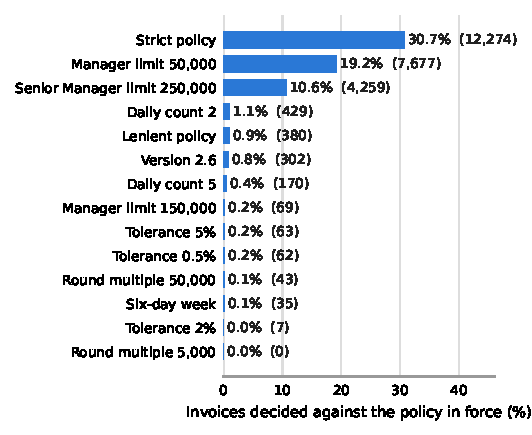
\includegraphics[width=\columnwidth]{fig_policy_change.pdf}
\caption{Share of the 40{,}000 invoices that a system with thresholds frozen at version 2.5 decides against the policy in force, for each policy variant. The policy-driven controls decide none against it.}
\label{fig:policychange}
\end{figure}

\textit{In the application.} We repeated one change through the deployed path. On the ledger of 20{,}000 invoices, audited under version 2.5, 240 invoices awaited review and 300 findings were stored. After the strict policy document was adopted with one command and the ledger audited again, 6{,}353 invoices awaited review and 6{,}546 findings were stored, 6{,}060 of them under the approval-limit clause. Adopting the document took 7 seconds and the audit of 20{,}000 invoices, with every result, finding and trail entry stored, took one minute on a laptop. No file of the system was edited between the two runs.

\textit{Throughput.} In memory, the controls audited 560{,}000 invoices in 13 seconds in a single process (about 44{,}000 invoices per second on an Intel i5-1235U), without any model call.

\subsection{Discussion and Limitations}
The adherence of 1.000 must be read for what it is. The controls and the ground truth are two implementations of the same written rules by the same authors; that they agree on every invoice under every policy shows that each document was read correctly and that no control keeps a threshold of its own. It is a verification of the mechanism, not a detection result, and it says nothing about whether the rules are the right ones.

The quantities that are not fixed by construction are those of the frozen system. They show that ordinary revisions of a procurement policy move between a handful and a third of the decisions on these ledgers, and that a tightening turns into missed escalations. A system that must be edited by hand to follow its policy carries this risk for as long as the edit is late or wrong.

Four limits apply. First, pattern extraction reads only the wording of one template and refuses other documents with reasons. A model-assisted path for policies in their own wording was measured separately on six short documents: a local 7B model proposed 80 of 84 values correctly, a check by code verified 56 of them and held back 24 right ones for the reviewer, and two wrong values passed the check, so the confirming person remains a required safeguard. Second, the system executes only rules for which it has a control; a new kind of rule needs a new control. Third, the ledgers are synthetic, so the counts describe how these ledgers react to these changes and not the books of a particular organisation. Fourth, the experiment covers the twelve rule-defined clauses; the four judgement clauses are assigned to language-model agents, which have been run only in a pilot of 20 invoices and whose accuracy we have not yet measured.

\end{document}
